\documentclass[a4paper, 12pt]{article}


\usepackage{amsmath,amsthm,amssymb}
\usepackage[T1,T2A]{fontenc}
\usepackage[utf8]{inputenc}
\usepackage[english,russian]{babel}
\usepackage{array}

\usepackage{tikz}
\usepackage{dsfont}
\usepackage{cancel}
\usepackage{ulem}
\usepackage{csquotes}

\usepackage{graphicx}%Вставка картинок правильная
\usepackage[caption=false]{subfig}
\usepackage[export]{adjustbox}
\usepackage{float}%"Плавающие" картинки
\usepackage{wrapfig}%Обтекание фигур (таблиц, картинок и прочего)

\usepackage{hyperref}
\hypersetup{
	colorlinks = true,
	linkcolor = black,
	filecolor = black,
	urlcolor = black,
	citecolor = black,
	% pdftitle={Отчёт по учебной практике, Андреев Иван Николаевич, 22.Б27-фз.},
	% pdfpagemode=FullScreen,
}

\usepackage{multirow}
\usepackage{colortbl}

\usepackage{spbu-ff-3kurs}
\usepackage[style=gost-numeric,language=auto,autolang=other,sorting=none,backend=biber]{biblatex}
\addbibresource{refs.bib}

\newcommand{\Rarr}{\Rightarrow}
\newcommand{\rarr}{\rightarrow}
\newcommand{\Lrarr}{\Leftrightarrow}
\newcommand{\ths}{\thinspace}
\newcommand{\ptl}{\partial}
\newcommand{\defis}{— }
\newcommand{\degg}{º}
\newcommand*\circled[1]{\tikz[baseline=(char.base)]{
		\node[shape=circle,draw,inner sep=2pt] (char) {#1};}}

\usepackage{mhchem}
\usepackage{chemfig}

\usepackage{slashbox}

\usepackage{setspace}
% \onehalfspacing{} % Полуторный интервал
%% или
%\doublespacing  % Двойной интервал
%% или
% \setstretch{1.5} % Произвольное значение (например, 1.25)

%%%%%%%%%%%%%%%%%%%%%%%%%%%%%%%%%%%%%%%%%%%%%

\begin{document}
\FirstPage{03.03.01 «Прикладные физика и математика»}
{22.Б27-фз}{Шишкевич Даниил}
{с.н.с., к.ф.-м.н.}{Сыч Томаш Сергеевич}
{с.н.с., к.ф.-м.н.}{Ксенофонтов Александр Андреевич}
{2026}

\ToC{}

\begin{onehalfspace}
\section*{Введение}
\addcontentsline{toc}{section}{ВВЕДЕНИЕ}

	Ионы тяжелых металлов (в частности, меди ($Cu^{2+}$) и никеля ($Ni^{2+}$)) являются распространенными загрязнителями водных экосистем и представляют серьезную угрозу для здоровья человека и окружающей среды \cite{find_ref}.
	Хотя медь необходима организму человека в качестве микроэлемента, ее избыток может приводить к острым и хроническим заболеваниям, как желудочно-кишечные расстройства, поражения печени и почек \cite{find_ref}.
	Никель классифицируется как потенциальный канцероген и вызывает аллергические реакции, респираторные заболевания и системное отравление \cite{Yang:2014}.
	Международные организации и национальные органы здравоохранения установили строгие нормы содержания этих элементов в питьевой воде.

	На протяжении нескольких десятилетий для определения концентрации ионов тяжелых металлов применялись различные аналитические методы.
	К стандартным инструментальным методам относятся атомно-абсорбционная и эмиссионная спектроскопия, хроматография, а также сенсорные системы (включая электрохимические и колориметрические подходы) \cite{Elkhatat:2021, Zhou:2024}.
	Эти методы обеспечивают высокую чувствительность и селективность, позволяя одновременно определять различные элементы в следовых количествах.
	Однако такие подходы имеют существенные ограничения, которые сдерживают их широкое применение.
	Прежде всего, эти методы требуют дорогостоящего, сложного оборудования и высококвалифицированного персонала для интерпретации результатов.
	Кроме того, аналитическая процедура включает длительные этапы подготовки проб, которые требуют использования агрессивных реагентов и специализированной лабораторной инфраструктуры.
	Это делает невозможным проведение анализа на месте или в полевых условиях и требует транспортировки проб в централизованные аналитические лаборатории.
	Помимо спектроскопических методов, для определения ионов металлов используются электрохимические методы (такие как вольтамперометрия и потенциометрия).
	Электрохимические методы отличаются простотой эксплуатации, быстрым временем анализа и возможностью одновременного определения нескольких ионов.
	Однако они часто оказываются дорогостоящими и недостаточно селективными, особенно в присутствии ионов-интерферентов в пробах природной воды.
	Кроме того, загрязнение электродов и пассивация поверхности могут привести к некорректным результатам подобного исследования \cite{Bond:1983}.

	В последние годы интенсивное развитие было направлено на применение флуоресцентных наносенсоров для определения ионов тяжелых металлов.
	Флуоресцентные методы обладают рядом существенных преимуществ: высокой чувствительностью, возможностью обнаружения в реальном времени, низкой стоимостью анализа и простотой эксплуатации.
	Флуоресцентные зонды демонстрируют быструю реакцию на присутствие целевых аналитов, что позволяет использовать их в портативных аналитических устройствах.
	Кроме того, обнаружение на основе флуоресценции может быть легко реализовано с помощью коммерчески доступного оборудования или даже адаптировано для аналитических платформ на основе смартфонов \cite{Yang:2014}.
	В частности, широко распространено использование флуоресцентных металлических кластеров, стабилизированных различными биополимерными матрицами, в качестве сенсорных систем \cite{Song:2016,Ding:2021}.

	Золотые нанокластеры привлекли значительное научное внимание благодаря своим свойствам, таким как яркая люминесценция, высокая химическая стабильность и низкая токсичность \cite{Chakraborty:2017}.
	Золотые нанокластеры синтезируются с использованием различных методик, включая белки, пептиды, полисахариды и органические молекулы в качестве восстанавливающих и стабилизирующих агентов \cite{Ding:2021, Kawasaki:2011, Baksi:2013, Xavier:2010, Xie:2009}.
	Такой биомолекулярный подход к синтезу позволяет получать биосовместимые комплексы с контролируемым размером и люминесцентными свойствами.
	Флуоресцентные материалы на основе золотых нанокластеров демонстрируют увеличенное время жизни люминесценции и повышенную фотостабильность по сравнению с традиционными органическими красителями и квантовыми точками.
	Эти преимущества делают золотые нанокластеры особенно привлекательными для аналитических применений, где особенно важно иметь стабильный во времени сигнал люминесценции \cite{find_ref}.

	Белки и пептиды, как биомолекулярные стабилизаторы, играют ключевую роль в синтезе люминесцентных золотых кластеров.
	Используя аминокислотные остатки, такие как цистеин, триптофан и тирозин в качестве восстановителей, можно синтезировать высокофлуоресцентные кластеры в мягких условиях в водных растворах.
	Тирозин, обладающий фенольной группой, особенно эффективен в качестве стабилизатора для золотых наночастиц.
	Благодаря своим окислительно-восстановительным свойствам тирозин способен восстанавливать ионы $Au^{3+}$ до нейтральных ($Au^0$) при щелочном pH, одновременно стабилизируя образующиеся кластеры посредством координационных взаимодействий \cite{find_ref}.

	Настоящее исследование направлено на разработку простого, быстрого и экономически эффективного метода определения ионов меди в водных растворах на основе Tyr-AuNCs.
	Ключевым нововведением данной работы является демонстрация того, что стабилизированные тирозином золотые кластеры сохраняют свои флуоресцентные и сенсорные свойства после лиофилизации, что позволяет разработать готовый к использованию набор для определения концентрации ионов меди в образцах.
	Такой подход является новым, уникальным и существенно отличается от существующих методов тем, что обеспечивает простоту использования, а также исключает необходимость в специализированных дорогостоящих материалах и оборудовании.

\newpage

\section*{Литературный обзор}
\addcontentsline{toc}{section}{ЛИТЕРАТУРНЫЙ ОБЗОР}

	\subsection*{Золотые нанокластеры}
	\addcontentsline{toc}{subsection}{Золотые нанокластеры}

	В настоящее время наноматериалы находят своё применение во многих областях: медицине, фармацефтике, электронике и прочих.
	В более широком смысле эти материалы можно разделить на несколько категорий, основываясь на их размерах, поскольку это напрямую влияет на электронно-энергетические свойства объекта (см. рис. \ref{fig:el-en-pref}).

	\begin{figure}[h]
		\centering
		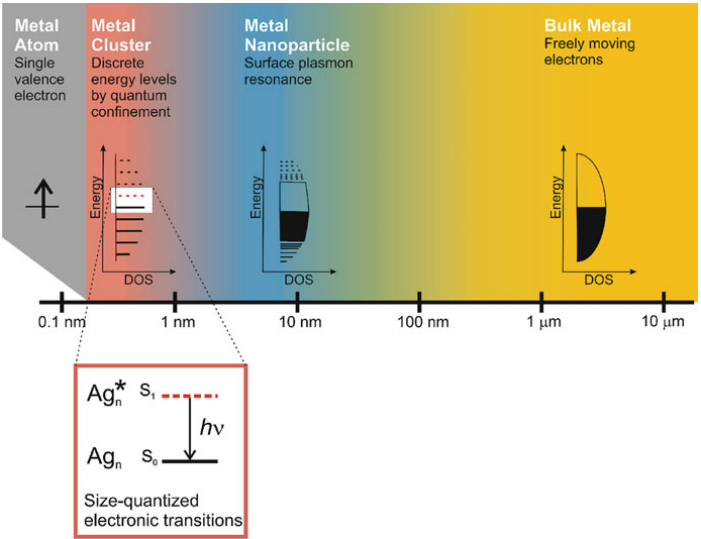
\includegraphics[width=0.75\linewidth]{attachments/struct.png}
		\caption{Сравнительная схема электронно-энергетических свойств металла в зависимости от его размера \cite{Díez2010}}
		\label{fig:el-en-pref}
	\end{figure}

	Когда размер наночастиц сравним с длиной волны света, используемой для возбуждения, т.е. $R \approx \lambda$, оптические свойства, проявляемые этими наночастицами, почти аналогичны тем, которые наблюдаются для объёмных металлов.
	Однако при уменьшении размера наночастиц, т.е. $R < \lambda$, их оптические характеристики становятся функцией их размера.

	Важное отличие нанокластеров от более крупных систем~- сверхмалый размер, не превосходящий 2-3 нанометров.
	Это отличие приводит к молекулярноподобным свойствам нанокластеров, таким как дискретные уровни энергии со значительной шириной запрещённой зоны, существенное поглощение с множеством одиночных электронных переходов, а также зависящая от их размера и поверхности фотолюминесценция.

	\subsection*{Синтез нанокластеров}
	\addcontentsline{toc}{subsection}{Синтез нанокластеров}

	Флуоресцентные свойства золотых нанокластеров сильно зависят от состава и окружения, а значит возможно получить требуемые свойсва путем вариации условий синтеза (концентрации металла и матрицы, pH, температура, время инкубации и т.д.)

	Изменение уровня pH приводит к протонированию (или депротонированию) функциональных групп на поверхности матрицы.
	Это напрямую влияет на процесс стабилизации кластера и его дальнейшие взаимодействие с другими молекулами.
	В статье \cite{sych:2024} авторами был получен стабилизированный тирозином золотой нанокластер, фотофизические свойства которого значительно изменялись при изменении pH при синтезе.

	Существует несколько стратегий получения фотолюминесцентных нанокластеров. Основными являются стратегии «сверху-вниз» и «снизу-вверх».
	В то время как первая подразумевает под собой создание наноматериалов за счёт уменьшения размеров крупных врагментов и не влечёт за собой образование наночастиц в качестве побочного продукта, вторая стратегия основывается на восстановлении ионов металла (золота в данной работе) с их последующей агрегацией в кластеры в присутствии стабилизирующего агента.
	Стратегия «снизу-вверх» можно реализовать различными методами, такими как: фотовосстановление, электрохимия, сонохимия, микроволновый синтез и синтез на стабилизирующей матрице.

	Наиболее распространенный матричный синтез как раз и был использован в данной работе. Более того, рассмотренный L-тирозин выполняет роль не только матрицы, но и восстанавливающего агента, т.е. восстанавливает ионы металла до нулевого валентного состояния. В результате подобной процедуры мы получаем комплекс тирозина с металлом в нулевом валентом состоянии.

	\subsection*{Применение нанокластеров}
	\addcontentsline{toc}{subsection}{Применение нанокластеров}

\newpage
\section*{Материалы и методы}
\addcontentsline{toc}{section}{Материалы и методы}

	\subsection*{Используемые материалы}
	\addcontentsline{toc}{subsection}{Используемые материалы}

	В данной работе в качестве стабилизирующей матрицы использовалась аминокислота L-тирозин, поставляемая в лиофилизированном виде (SigmaAldrich, 60-18-4).
	Для приготовления растворов использовалась вода сверхвысокой степени очистки (SQ water, $R>18.2~M\Omega$).
	Остальные реагенты:
	гидроксид натрия~– $\text{NaOH}$ (1310-73-2),
	пентагидрат сульфата меди~– $\text{CuSO}_4$ (7758-99-8),
	хлорид никеля~– $\text{NiCl}_2$,
	тригидрат тетрахлораурата водорода (16961-25-4)~– $\text{HAuCl}_4$
	~– приобретены в Sigma-Aldrich.

	\subsection*{Экспериментальные методы}
	\addcontentsline{toc}{subsection}{Экспериментальные методы}

		\subsubsection*{Спектроскопия поглощения}
		\addcontentsline{toc}{subsubsection}{Спектроскопия поглощения}

		Методы оптической спектроскопии используются для исследования влияния образца на пропущенное через него излучение. При этом рассматриваетя видимый диапазон длин волн, а также ближние ультрафиолетовый (УФ) и инфракрасный (ИК) диапазоны.

		В исследованиях биополимеров часто рассматривают процесс поглощения излучения, который показывает на каких длинах волн происходят переходы из основного электронного состояния на возбужденные уровни. Так как поглощение света связано с электронными переходами между энергетическими уровнями, то спектроскопия поглощения является хорошим инструментом для количесвенного и качественного анализа веществ.

		Примером теоретической зависимости, которая хорошо описывает процесс поглощения и широко используется н практике, является закон Бугера-Ламберта-Бера (см. формулу \ref{eq:BLB-law}):

		\begin{equation}
			I=I_0\exp(-\varepsilon_\lambda Cl),
			\label{eq:BLB-law}
		\end{equation}

		где $I$ - интенсивность света после прохождения через вещество, $I_0$ - начальная интенсивность света, $\varepsilon_\lambda$ - молярный коэффициент поглощения ($\text{л}\cdot\text{моль}^{-1}\cdot\text{см}^{-1}$) на длине волны $\lambda$, $C$ - концентрация вещества ($\text{моль}\cdot\text{л}^{-1}$), $l$ - толщина слоя вещества ($\text{см}$). Также вводится понятие оптической плотности $D$, которая выражается следующим образом (формула \ref{eg:opt-density}):

		\begin{equation}
			D=\log_{10}\frac I {I_0} = \varepsilon_\lambda Cl
			\label{eg:opt-density}
		\end{equation}

		Важно отметить, что для выполнения описанного закона необходим ряд условий: монохроматичность падающего излучения, параллельность падающего пучка света и наличие поглощающей в искомом диапазоне длин волн среды.

		Для регистрации спектров поглощения использовался двухлучевой сканирующий спектрофотометр УФ-видимого диапазона - Specord 210 Plus (Analytic Jena AG) – позволяющий регистрировать спектры в диапазоне длин волн от 190 до 1100~нм. Спектры записываются с использованием кварцевой кюветы, а коррекция производится на референсный сигнал от растворителя образца в той же кювете.

		\subsubsection*{Спектроскопия люминесценции}
		\addcontentsline{toc}{subsubsection}{Спектроскопия люминесценции}

		Люминесценция – это излучение атомами, молекулами, ионами и другими более сложными образованиями в ультрафиолетовой, видимой и ближней инфракрасной областях электромагнитного спектра, возникающее при переходе этих частиц из возбуждённого состояния в основное.
		Различают множество видов люминесценции в зависимости от типа возбуждающего воздействия.
		В частности, свечение вещества, вызванное действием на него света (УФ и видимый диапазоны), принято называть фотолюминесценцией.

		В основе фотолюминесценции лежат процессы квантовой механики, связанные с переходами электронов между электронными энергетическими уровнями в молекулах вещества. Эти процессы подразделяются на два основных типа, в зависимости от природы основного и возбуждённого состояний молекул: флуоресценцию и фосфоресценцию (см. рис.~\ref{Jablonski}).

		\begin{figure}
			\centering
			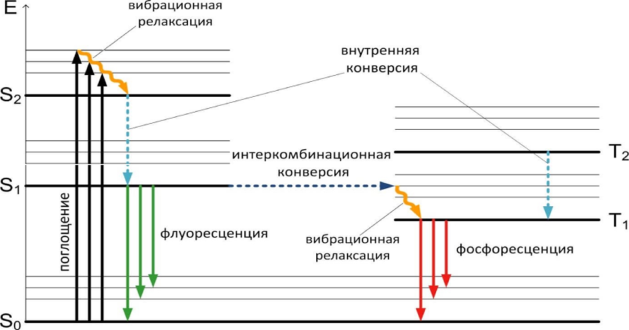
\includegraphics[width=1\linewidth]{attachments/Janlonski.png}
			\caption{Диаграмма Яблонского}
			\label{Jablonski}
		\end{figure}

		Флуоресценция возникает, когда молекула переходит из возбуждённого синглетного состояния в основное. В синглетном возбуждённом состоянии спины электрона на энергетически более высокой орбитали и электрона на более низкой энергетической орбитали имеют противоположную ориентацию (спаренные электроны). При возвращении электрона из возбуждённого синглетного состояния в основное, ориентация его спина не изменяется, и происходит процесс испускания кванта света. Этот процесс разрешен с точки зрения квантовой механики и характеризуется коротким временем жизни возбуждённого состояния, обычно от единиц микро- до единиц наносекунд.

		Фосфоресценция, напротив, связана с переходом молекулы из возбуждённого триплетного состояния в основное. Переход из возбуждённого триплетного состояния в основное требует изменения ориентации спина электрона, что является квантовомеханически «запрещённым» процессом, поэтому фосфоресценция характеризуется значительно большим временем жизни возбужденного состояния: от единиц милли- до сотен секунд.

		Добавление некоторых соединений к люминофору могут сильно изменить его фотофизические свойства, т.е. привести к усилению или тушению люминесценции.

		Уравнение Штерна-Фольмера является фундаментальным инструментом для анализа процессов тушения флуоресценции и описывает зависимость квантового выхода или интенсивности люминесценции от концентрации тушителя. В классической форме уравнение записывают, как:
		\begin{equation}
			I_0 / I = 1+K_{\text{дин}}[Q],
		\end{equation}
		где $I_0$ и $I$ -  интенсивности флуоресценции в отсутствие и в присутствии тушителя соответственно, $K_{\text{дин}}$ - константа динамического тушения, $[Q]$ - концентрация тушителя.

		Существует два основных механизма тушения люминесценции: динамическое и статическое.
		Динамическое тушение происходит за счёт столкновений возбужденных молекул флуорофора с молекулами тушителя в течение времени жизни возбужденного состояния. При этих столкновениях происходит безызлучательное возвращение молекулы в основное состояние, что снижает интенсивность и время жизни люминесценции. Важной характеристикой динамического тушения является зависимость времени жизни возбужденного состояния от концентрации тушителя — при увеличении концентрации время жизни уменьшается.

		Статическое тушение связано с образованием в основном состоянии неактивных люминесцирующих комплексов между молекулами флуорофора и тушителя. Такие комплексы не способны к флуоресценции, поэтому наблюдается снижение интенсивности излучения без изменения времени жизни возбужденного состояния. Время жизни остаётся постоянным или уменьшается, что позволяет отличить статическое тушение от динамического экспериментально. Статическое тушение проявляется в виде нелинейной зависимости интенсивности от концентрации тушителя и связано с равновесием образования комплексов

		\subsubsection*{Измерение времени жизни люминесценции}
		\addcontentsline{toc}{subsubsection}{Измерение времени жизни люминесценции}

		Временем жизни люминесценции принято считать средний промежуток времени, в течение которого молекула находится в возбужденном состоянии до того момента, как она вернется в основное состояние с испусканием фотона.

		Значение времени жизни люминесценции зависит от свойств самого объекта, его окружающей среды, температуры, а также от присутствия компонентов, которые могут либо подавлять, либо усиливать люминесценцию. Измерение времени жизни позволяет получить важную информацию о динамике переходов между энергетическими уровнями. Обладая этими данными, можно оценить эффективность процессов передачи энергии и взаимодействия с окружающей средой, а также изучить механизмы тушения (как динамического, так и статического).

		Существует два основных метода измерения времени жизни люминесценции: фазово - модуляционный и импульсный (временной). В фазово-модуляционном методе возбуждающий свет модулируется по интенсивности с заданной частотой. Затем измеряются сдвиг фазы и изменение амплитуды люминесцентного сигнала относительно возбуждающего излучения, что позволяет вычислить время жизни. В импульсном методе образец возбуждается короткими световыми импульсами, после чего регистрируется спад интенсивности люминесценции во времени. Полученная кривая затухания аппроксимируется суммой экспоненциальных функций, из которой определяется время жизни. В нашем исследовании применялся именно импульсный метод.

		Измерения времён жизни люминесценции были произведены на модульном спектрофлуориметре Fluorolog 3 (Ресурсный центр СПбГУ «Оптические и лазерные методы исследования вещества», researchpark.spbu.ru/laser-rus).

\newpage
\section*{Результаты и обсуждение}
\addcontentsline{toc}{section}{Результаты и обсуждение}

\subsection*{Синтез золотых нанокластеров, стабилизированных тирозином}
\addcontentsline{toc}{subsection}{Синтез золотых нанокластеров, стабилизированных тирозином}

	Синтез золотых кластеров проводился согласно нижеописанному протоколу.
	В раствор тирозина (объем 1~мл, концентрация 0.1~мг/мл) добавлялся раствор тетрахлороаурата~(III) водорода (объем 2.75~мкл, концентрация~0.1 М). Полученная смесь инкубировалась при температуре $55^\circ \text{C}$ и постоянном перемешивании в течение 30~минут.

\subsection*{Характеризация кластера}
\addcontentsline{toc}{subsection}{Характеризация кластера}

	Полученный нанокластер золота, стабилизированный тирозином, обладает максимумом возбуждения на длине волны 315~нм и максимумом испускания - 405~нм.
	Пик поглощения системы приходится на 290~нм. Также отмечается заметное поглощение в области 520~нм, что сигнализирует об образовании золотых наночастиц в качестве побочного продукта реакции (см. рис.~\ref{fig:ex-em-abs}).

		\begin{figure}[H]
			\begin{minipage}[!t]{0.45\linewidth}
				\centering
				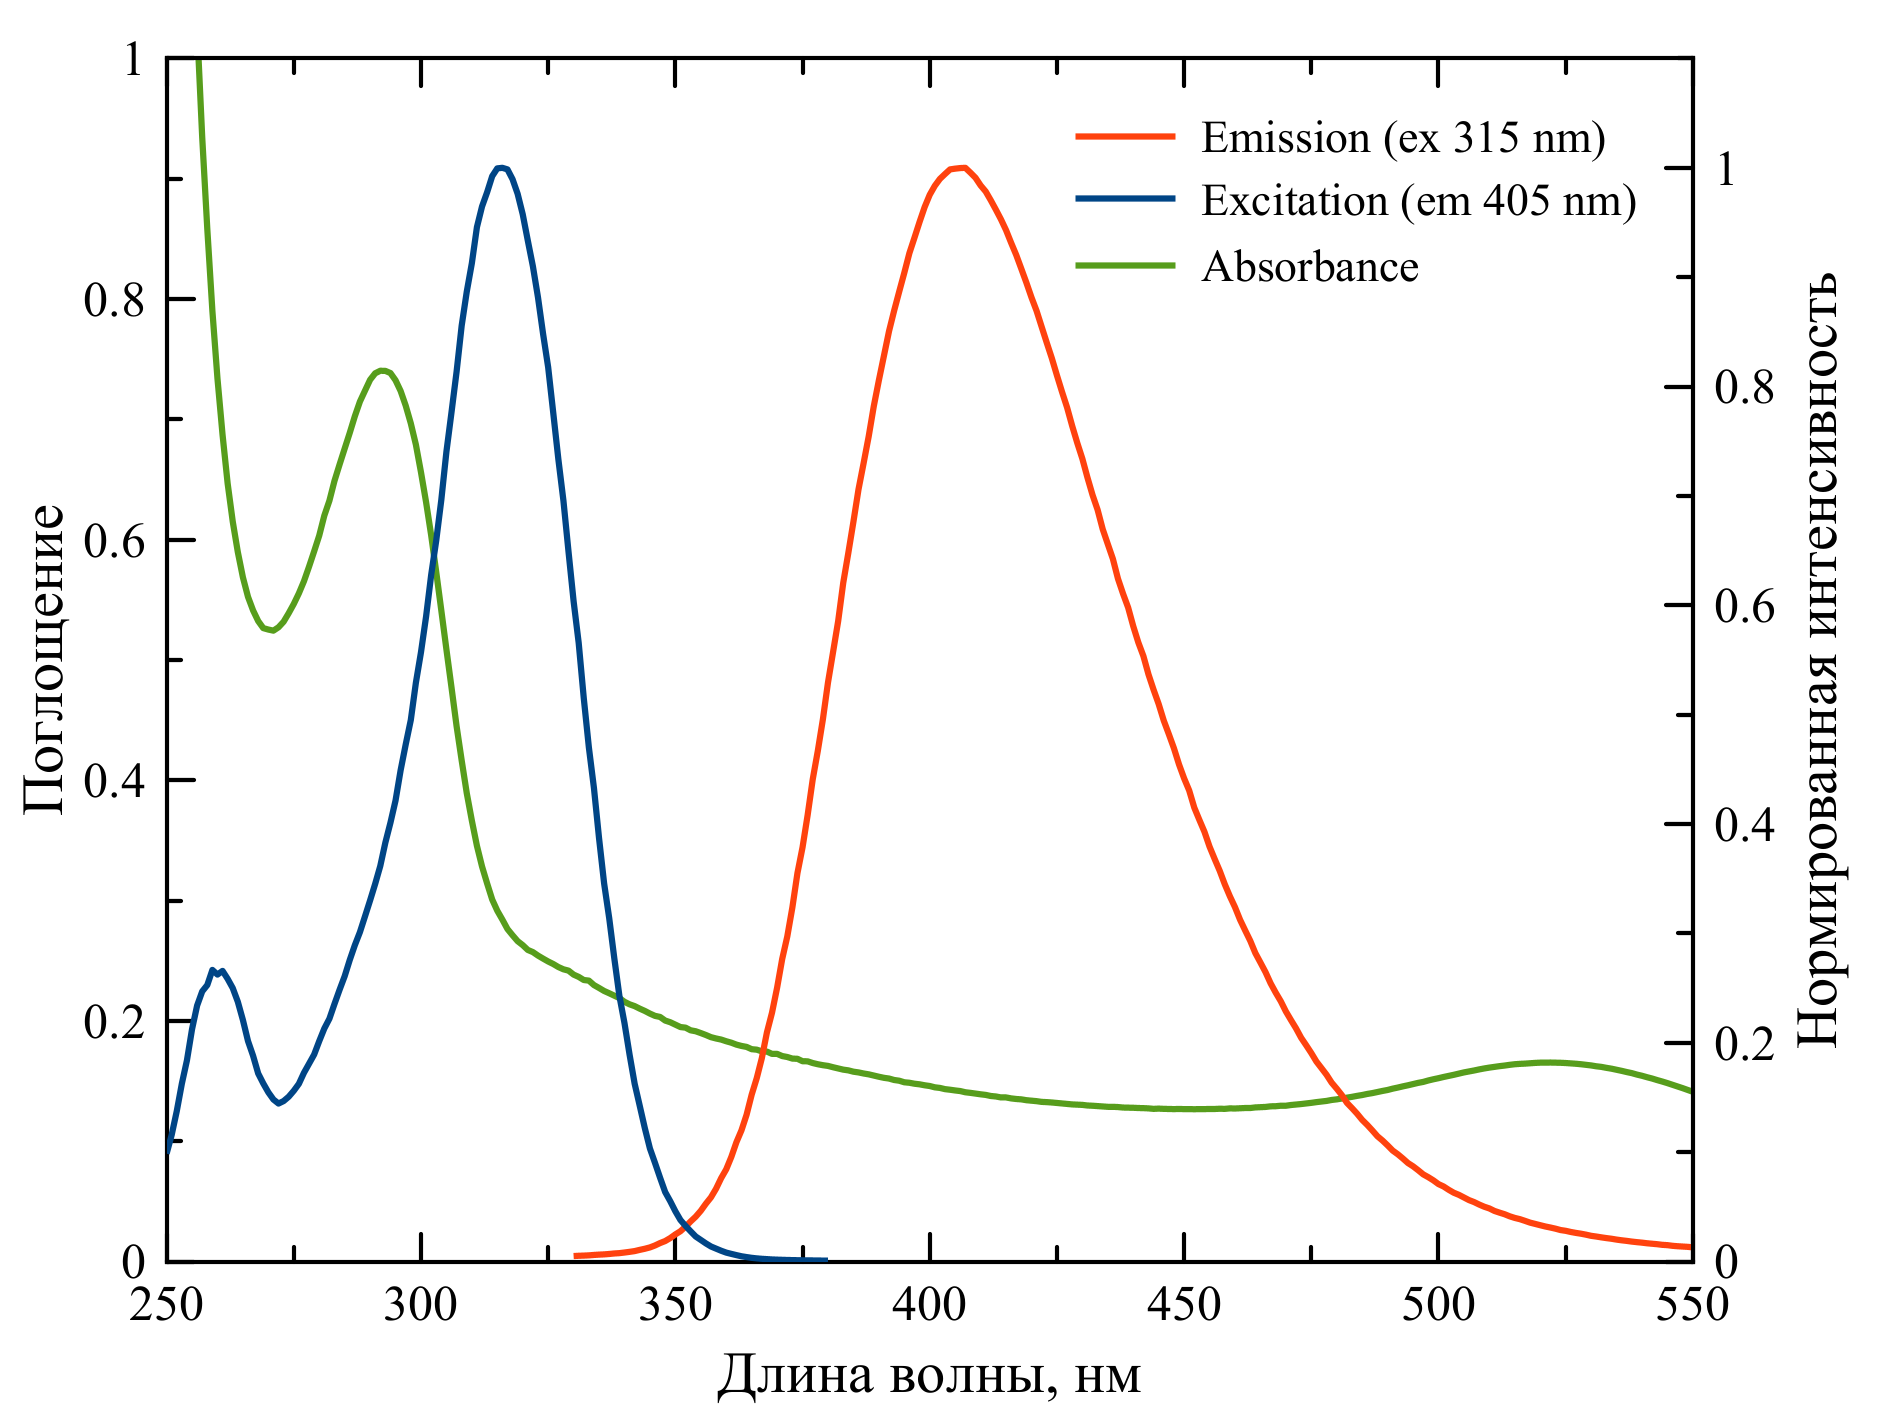
\includegraphics[width=\linewidth]{attachments/ex_em spectras.png}
				\caption{Спектры поглощения, возбуждения и испускания золотых нанокластеров}
				\label{fig:ex-em-abs}
			\end{minipage}
			\hfill
			\begin{minipage}[!t]{0.45\linewidth}
				\centering
				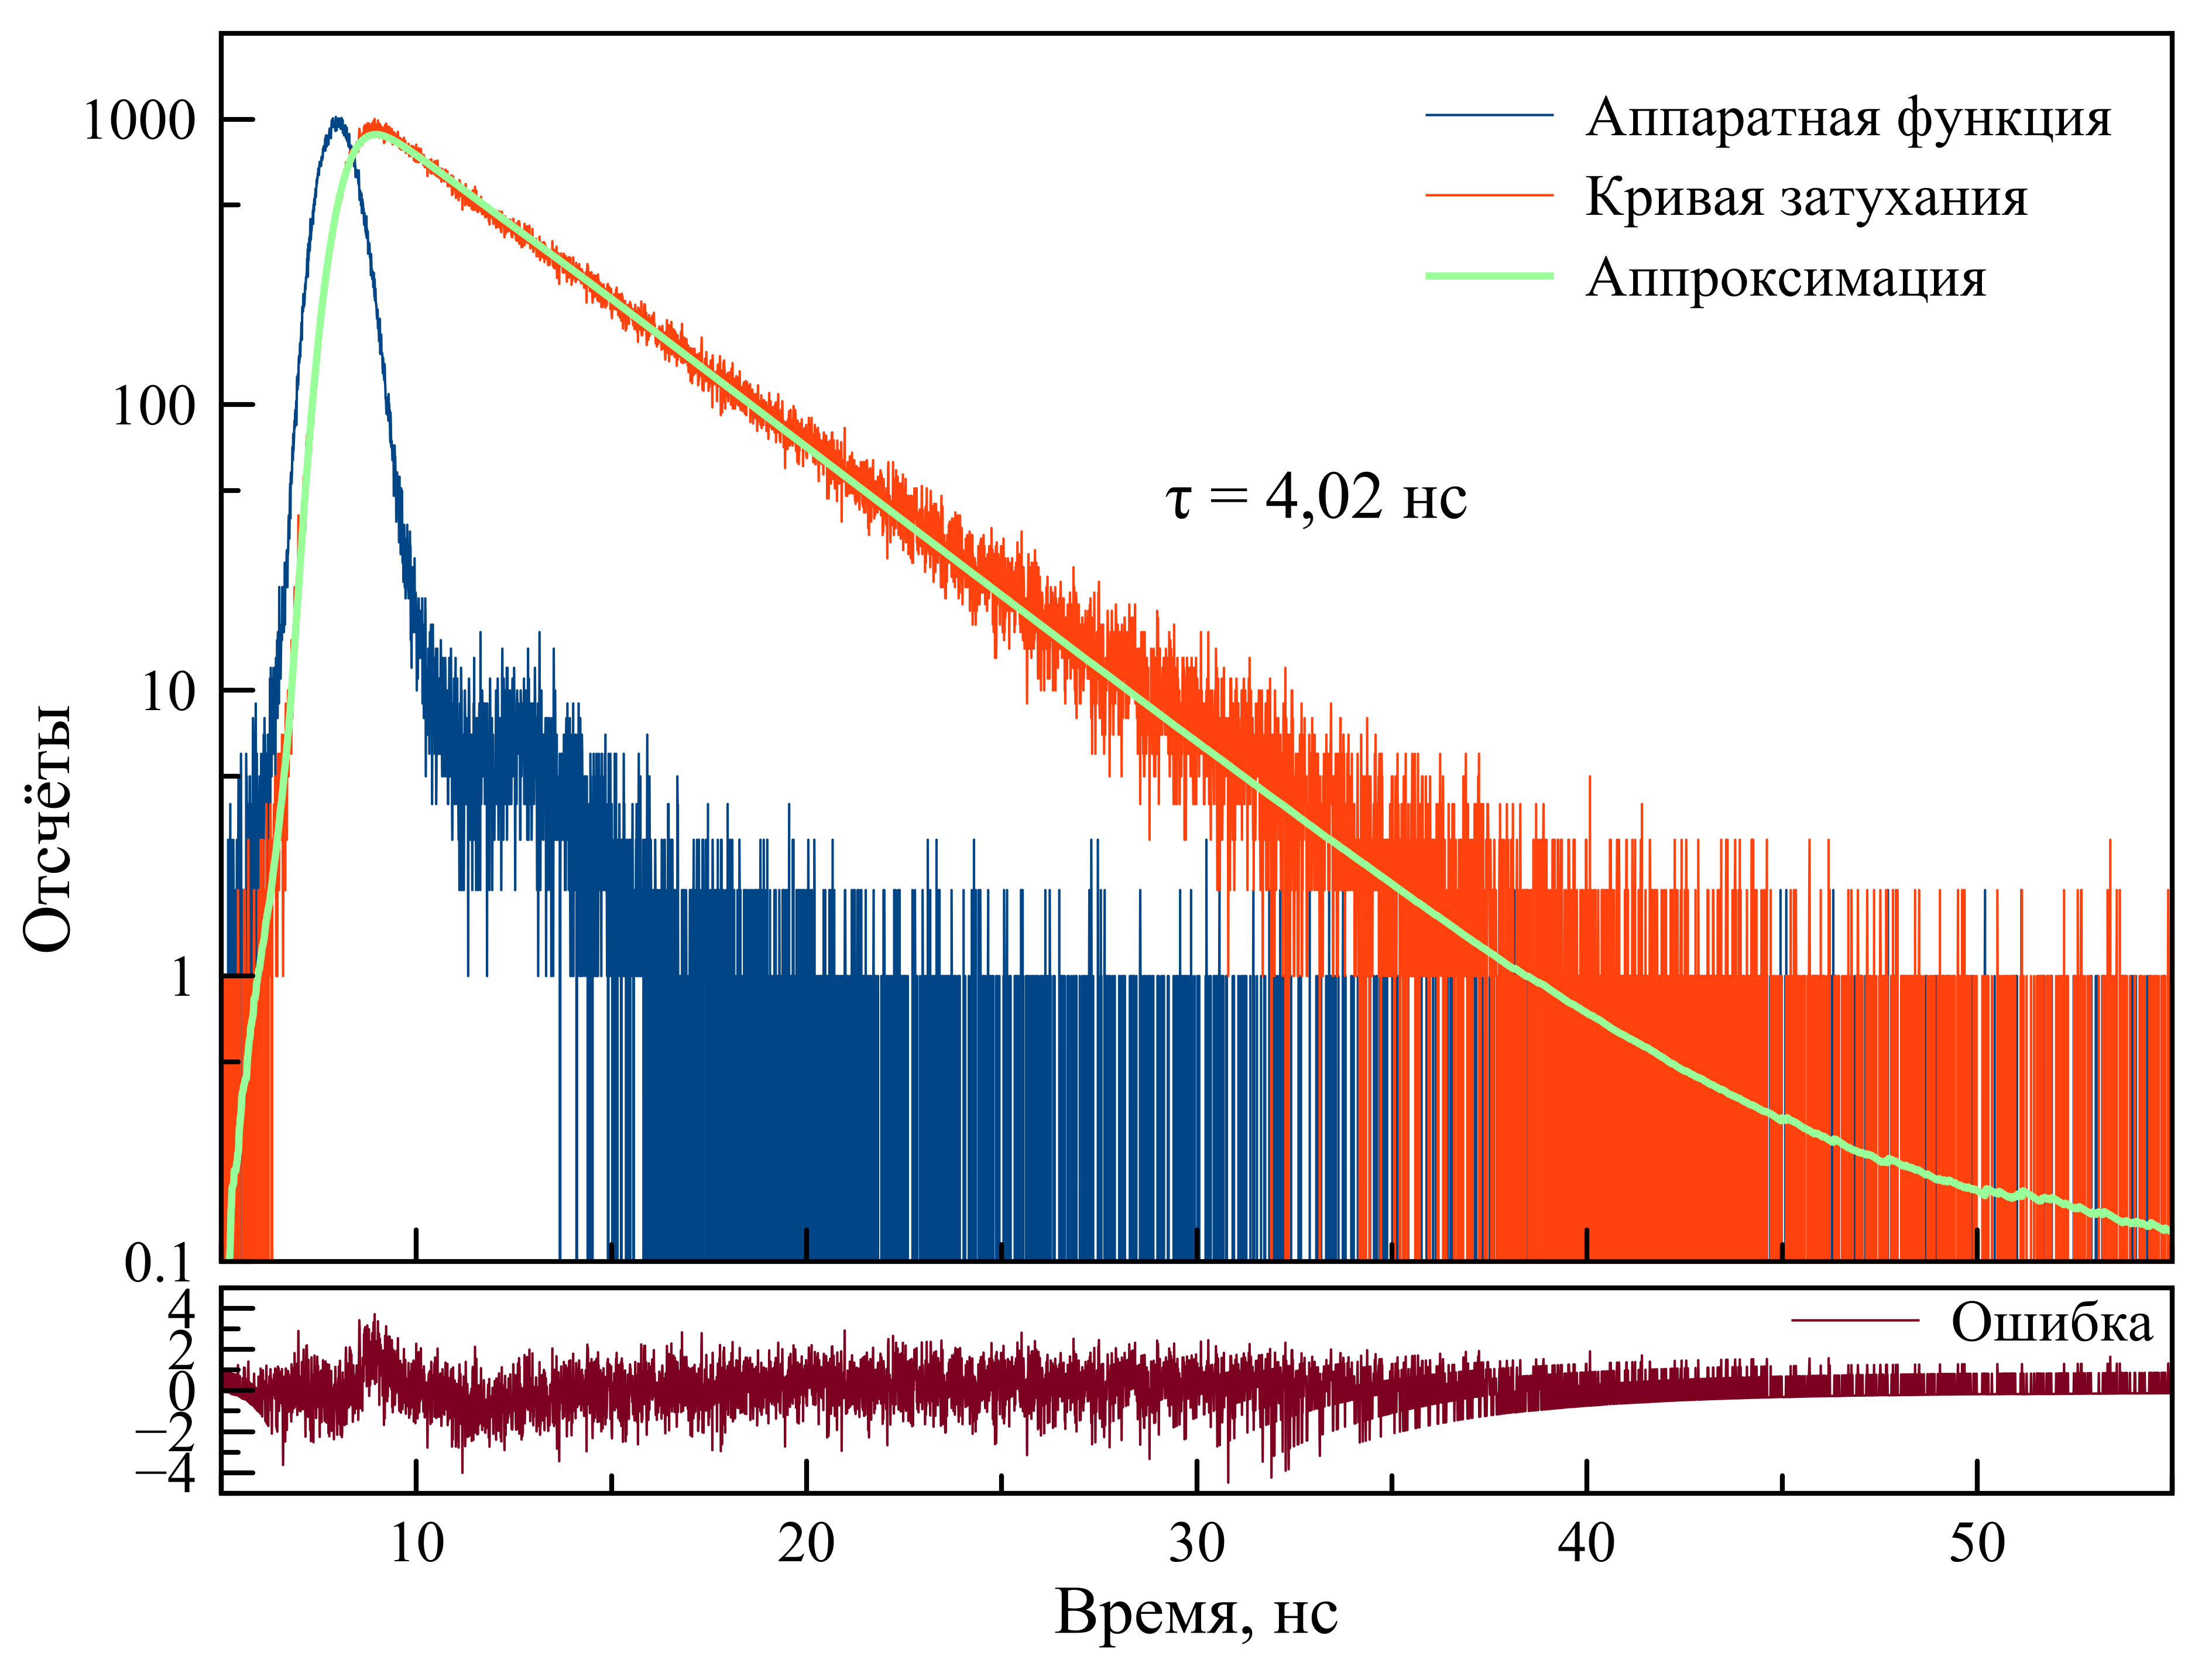
\includegraphics[width=\linewidth]{attachments/au lifetime.png}
				\caption{Кривая затухания люминесценции золотого нанокластера}
				\label{fig:au-TCSPC}
			\end{minipage}
		\end{figure}

	Также кластер был охарактеризован с точки зрения фотофизических характеристик, а именно было определено его время жизни, равное 4.02~нс (см. рис.~\ref{fig:au-TCSPC}), что согласуется с характерным для золотых нанокластеров значением.

\subsection*{Сенсорное применение кластера}
\addcontentsline{toc}{subsection}{Сенсорное применение кластера}

	К полученному золотому нанокластеру, стабилизированному тирозином, были добавлены различные аналиты - соли металлов натрия, калия, меди, цинка, никеля, цезия, кальция и серебра в концентрации 100~ммоль/л. Полученные образцы инкубировались в течение 15 минут при комнатной температуре и постоянном перемешивании.

	\begin{figure}[H]
		\centering
		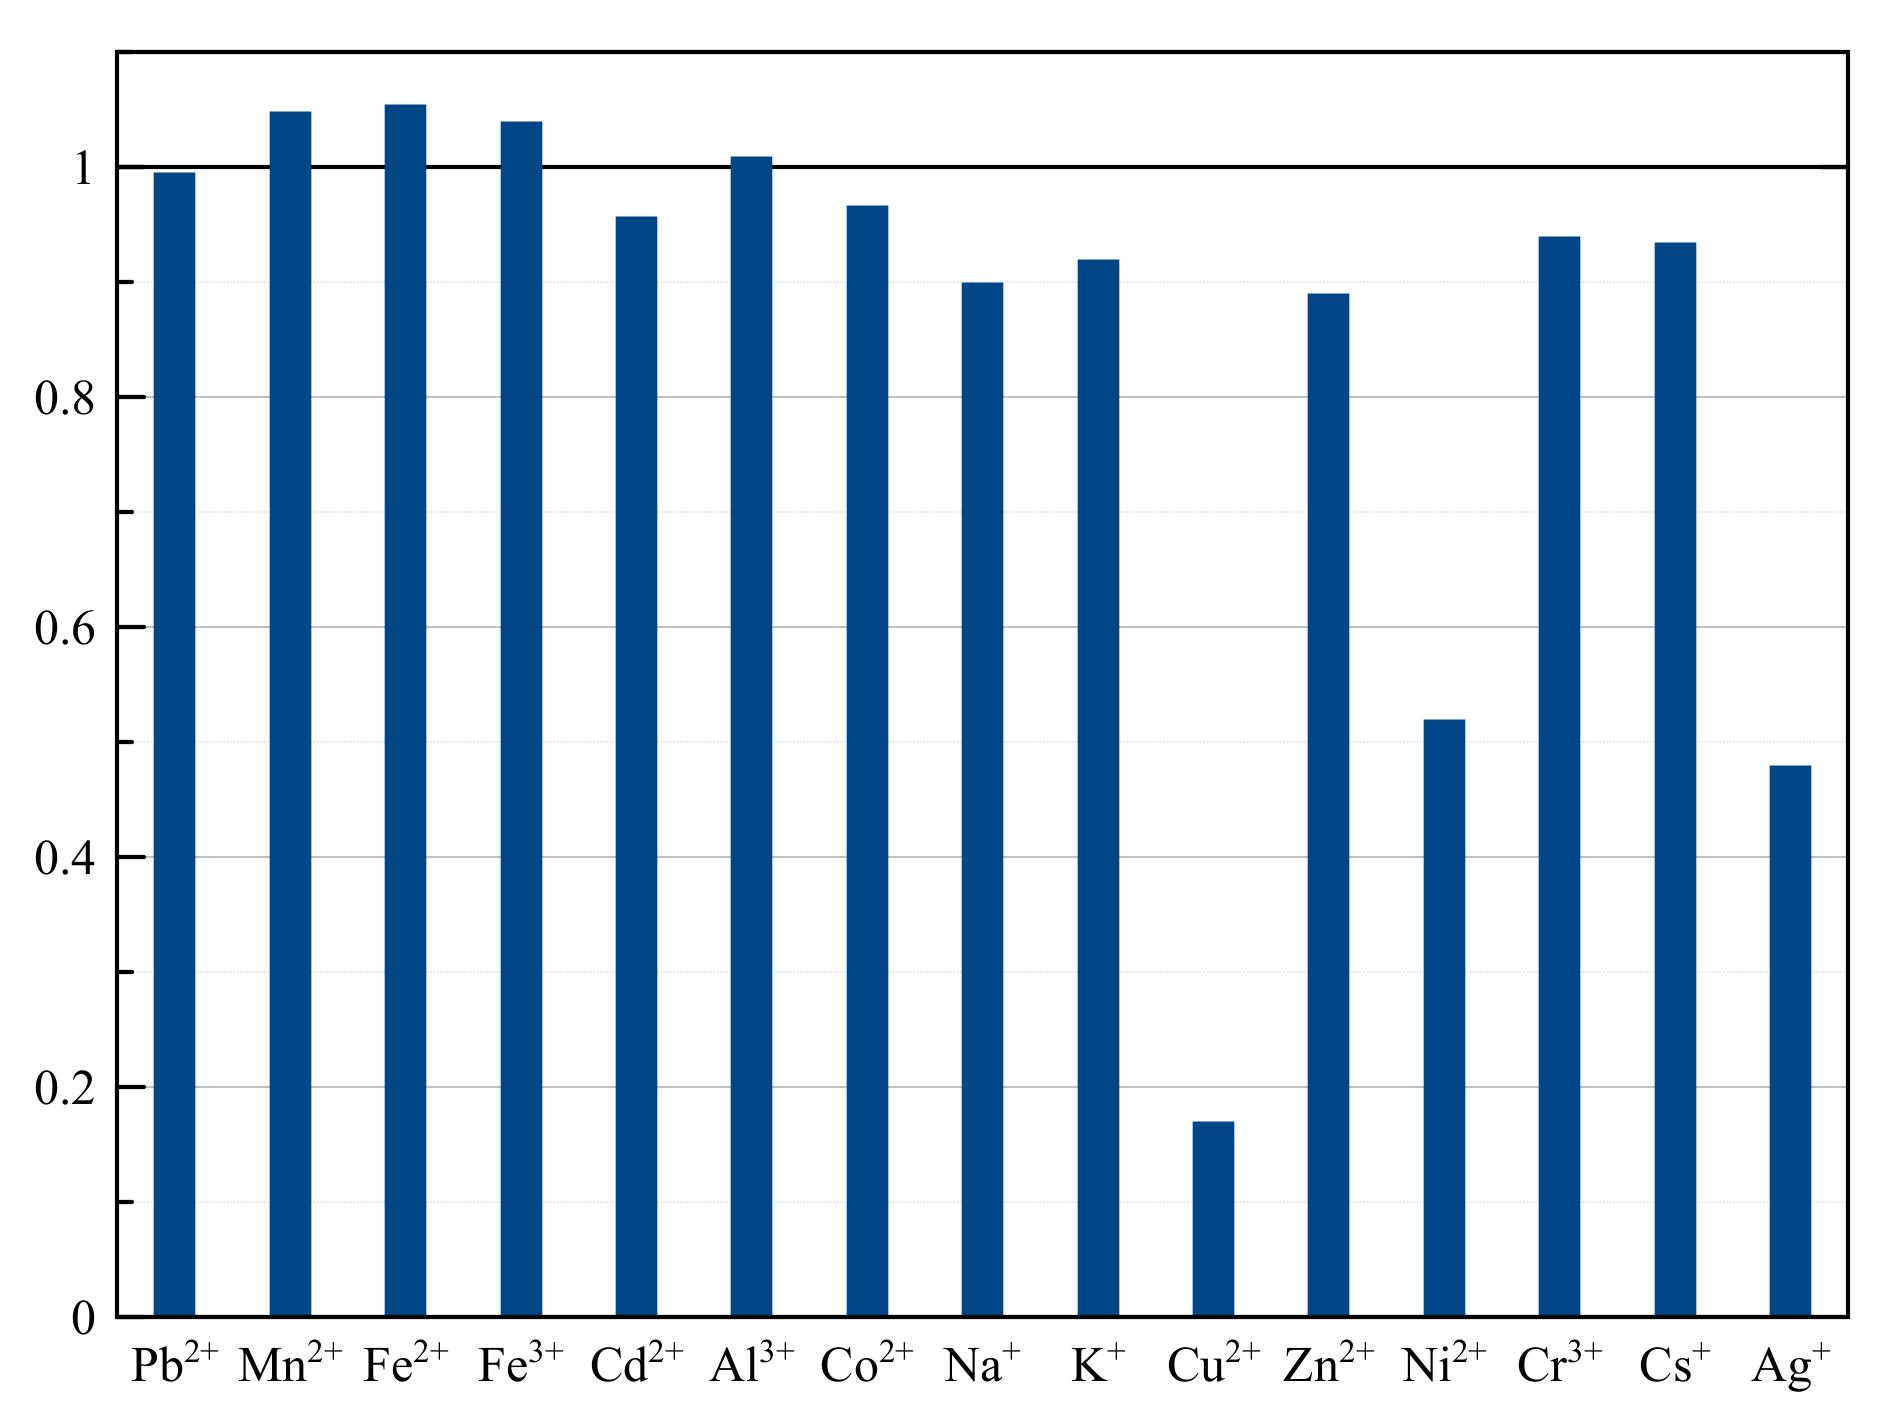
\includegraphics[width=0.75\linewidth]{attachments/image.png}
		\caption{Изменение люминесценции кластера в присутствии ионов металлов в концентрации 100 ммоль/л}
		\label{fig:react-est-ions}
	\end{figure}

	Было получено, что на люминесценцию кластера влияют не все представленные ионы (см. рис.~\ref{fig:react-est-ions}). Значительный эффект тушения люминесценции наблюдается только для ионов меди, никеля и серебра.

	\textbf{Штерн-Фольмер никель}

	\textbf{Штерн-Фольмер медь}

	\textbf{ПДК / ЛОД по прямым экспериментам}

	\textbf{Штерн-Фольмер медь лиоф}

	\textbf{TCSPC кластер}

	\textbf{TCSPC медь / никель}



\newpage
\section*{Заключение}
\addcontentsline{toc}{section}{ЗАКЛЮЧЕНИЕ}

\newpage
\section*{Благодарности}
\addcontentsline{toc}{section}{БЛАГОДАРНОСТИ}

Выражаю особую благодарность


\end{onehalfspace}
\newpage

% \section*{Список использованных литературных источников и информационных материалов}
\addcontentsline{toc}{section}{Список использованных литературных источников и информационных материалов}
% \bibliographystyle{unsrt}
\printbibliography[title={Список использованных литературных источников и информационных материалов}]


\end{document}